\subsection{Risultati e conclusioni}
Applicando la regola di classificazione descritta nel paragrafo precedente, ogni regione viene classificata ed i risultati vengono riportati direttamente sull'immagine come mostrato nella figura \ref{fig:GUIpostLBP}.

\begin{figure}[ht]
\begin{center}
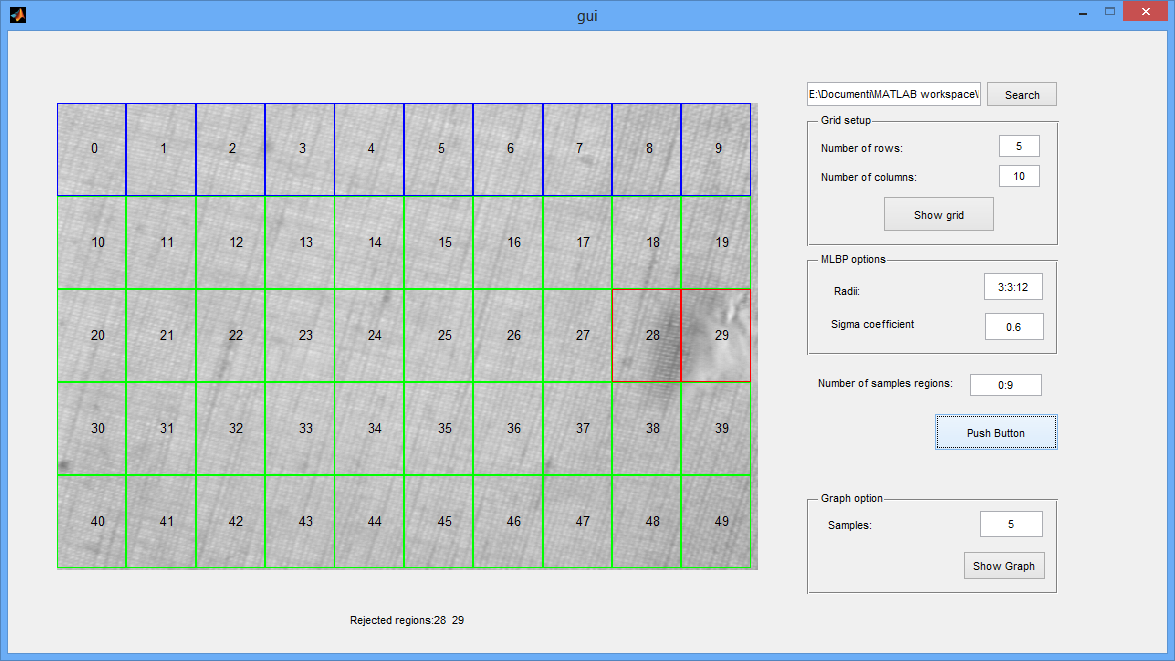
\includegraphics[width=.95\textwidth]{img/gui_post_lbp}
\caption{Risultati dell'operazione di classificazione. Le regioni con contorno di colore rosso sono quelle contenenti difetti, le regioni di colore blu sono quelle del training set e le regioni con contorno verde sono quelle ritenute corrette. }
\label{fig:GUIpostLBP}
\end{center}
\end{figure}

L'utente, cliccando sull'apposito bottone \textit{Show Graph}, può visualizzare i grafici delle distribuzioni gaussiane determinate precedentemente. In figura \ref{fig:worstGraph} è visualizzato un esempio dei grafici delle distribuzioni gaussiane delle cinque regioni con media $\mu_{test}$ peggiori.


\begin{figure}[ht]
\begin{center}
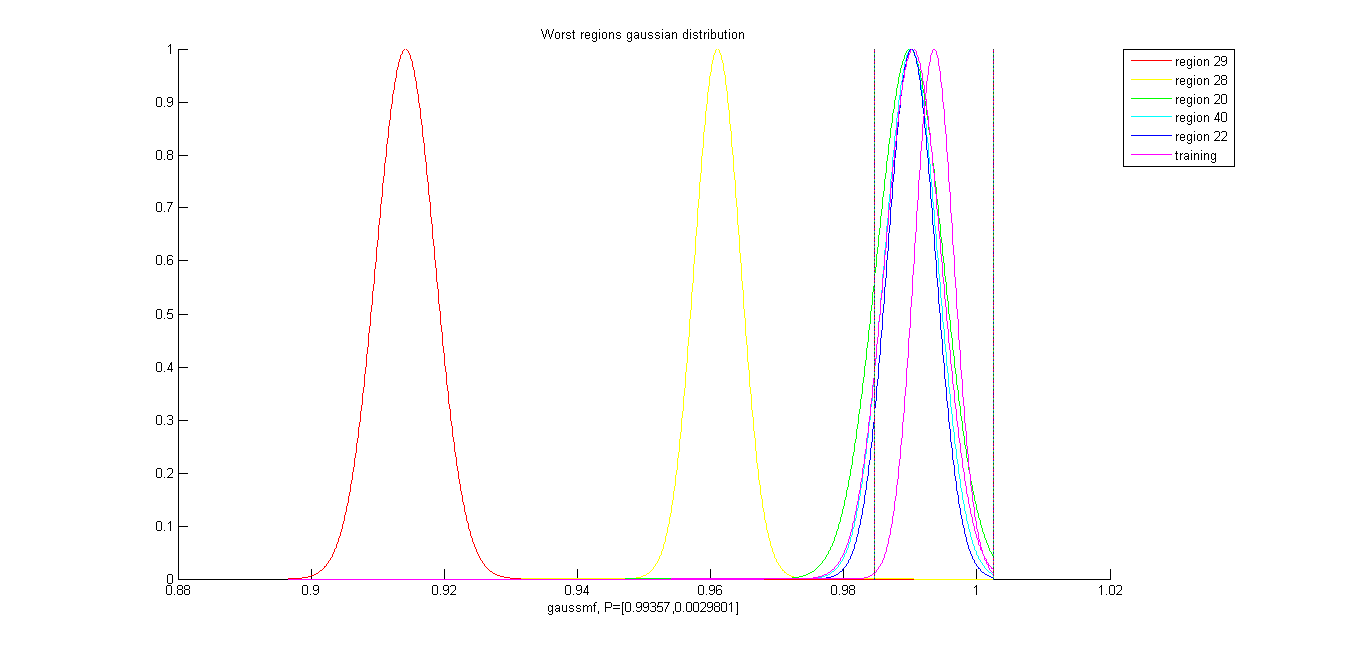
\includegraphics[width=1\textwidth]{img/worst_graph}
\caption{ Caso peggiore }
\label{fig:worstGraph}
\end{center}
\end{figure}


In figura \ref{fig:worstBestGraph}, è visualizzato un esempio dei grafici delle distribuzioni gaussiane delle cinque regioni con media $\mu_{test}$ peggiori tra quelle classificate come regioni corrette.


\begin{figure}[ht]
\begin{center}
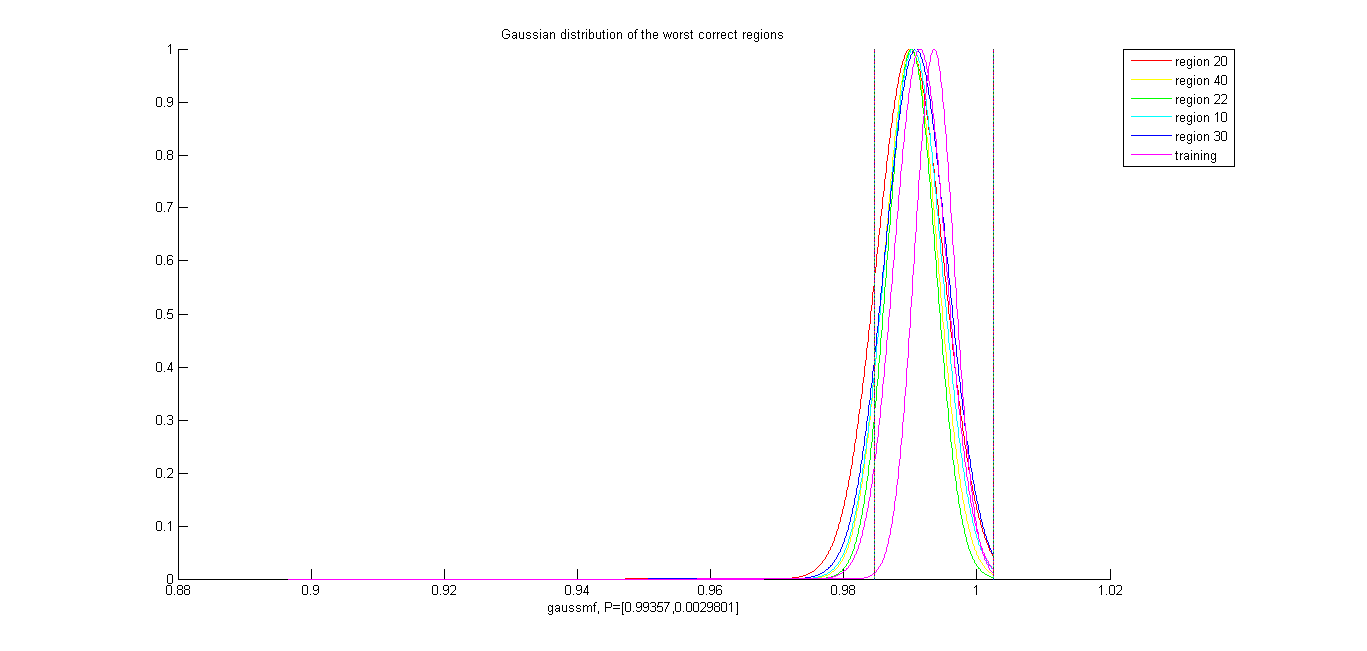
\includegraphics[width=1\textwidth]{img/worst_best_graph}
\caption{ I peggiori tra i migliori }
\label{fig:worstBestGraph}
\end{center}
\end{figure}

I risultati ottenuti in seguito all'applicazione del metodo da noi implementato su un numero significativo di immagini, si sono rivelati soddisfacenti. Infatti nei casi di classificazione di falsi positivi e veri negativi è bastato modificare opportunamente i parametri di configurazione per ottenere una classificazione esatta.